Para comprobar cómo se ajusta el modelo al comportamiento real de la emisión se tomaron medidas en el Laboratorio de Robótica 0L3 del Instituto de Computación Científica Avanzada de la Universidad de Extremadura (ICCAEx), situado en los Institutos Universitarios de Investigación de la Universidad de Extremadura en Badajoz.

En este laboratorio se dispone de una superficie amplia en la que fue posible usar un robot para automatizar la toma de medidas en divesos puntos, que más tarde fueron usados en la simulación colocando los receptores en dichos puntos.

\begin{figure}[H]
    \centering
    \begin{subfigure}[b]{0.45\textwidth}
        \centering
        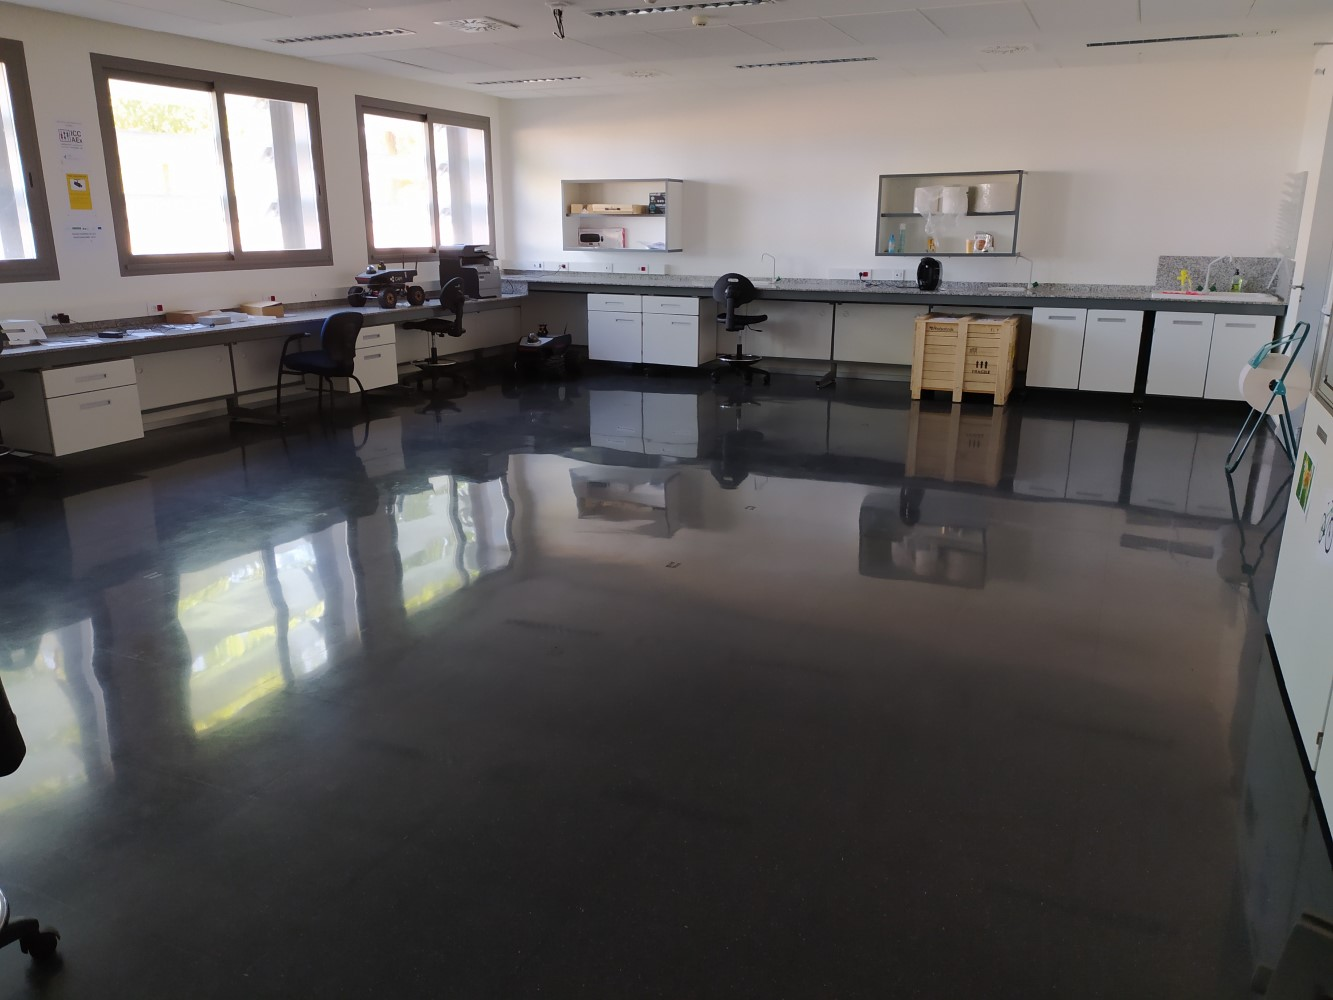
\includegraphics[width=6.8cm]{pic/lab1.jpg}
        % \caption{Imágenes de la antena del router utilizado.}
        % \label{fig:antena_router}
    \end{subfigure}
    ~~
    \begin{subfigure}[b]{0.45\textwidth}
        \centering
        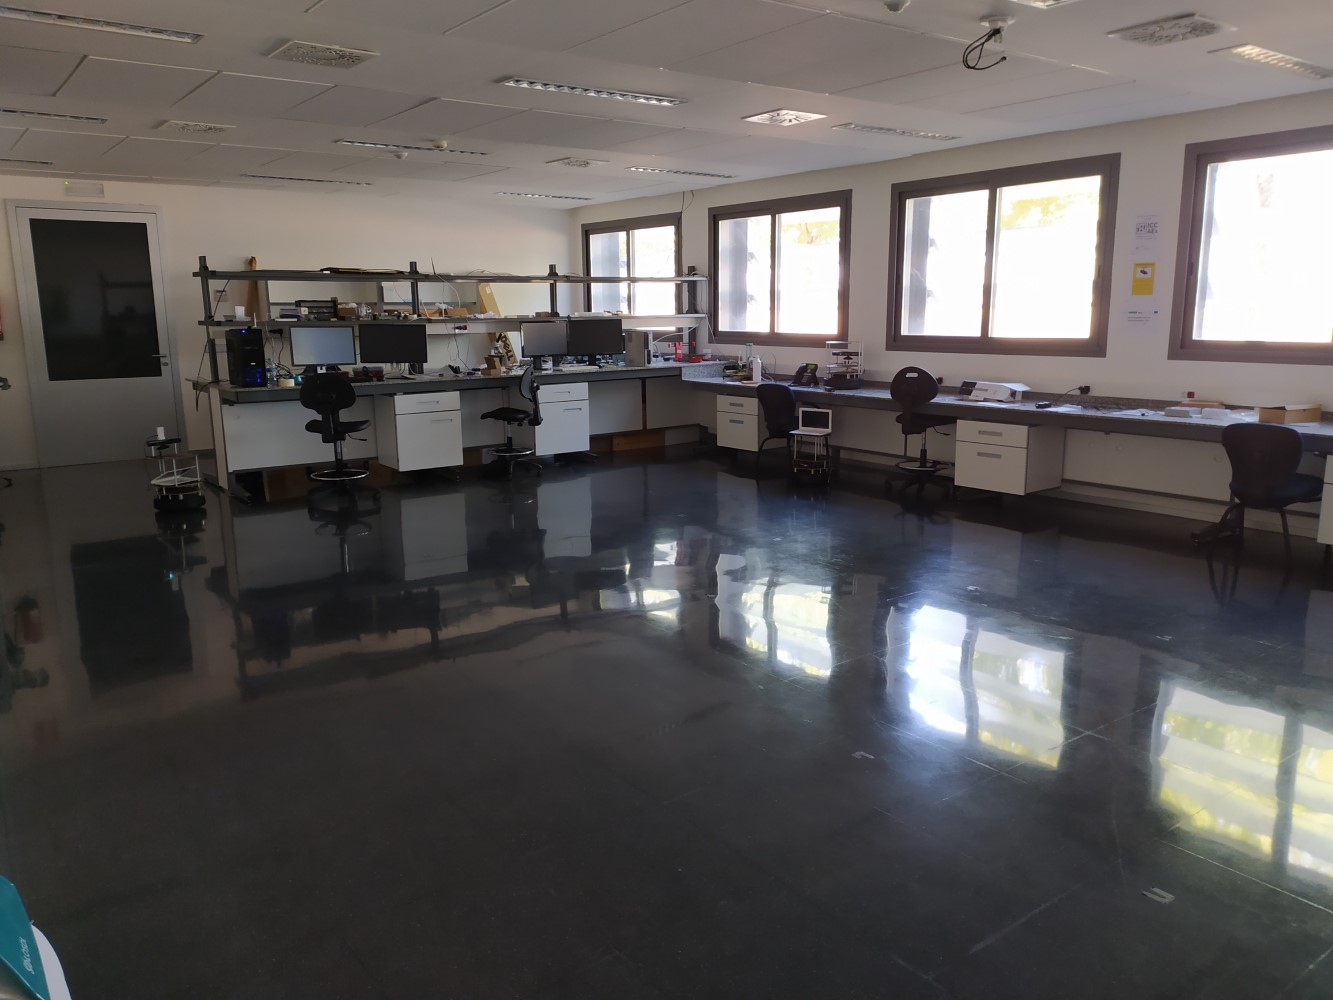
\includegraphics[width=6.8cm]{pic/lab2.jpg}
        % \caption{Imágenes de la antena receptora utilizada}
        % \label{fig:antena_receptor}
    \end{subfigure}
    \caption{Imágenes del laboratorio donde se realizaron las pruebas.}
    \label{fig:lab_pics}
\end{figure}


Cabe destacar que el entorno de pruebas tenía un especto electromagnético muy poblado.
Al encontrarse en un edificio con otros laboratorios, se encontraban entre 10 y 15 redes WiFi, con lo que resultó imposible encontrar algún canal libre para realizar las pruebas.

Para solventar esta contaminación se tomaron, para cada punto, 5 medidas esperando 5 segundos ente cada una de ellas, de modo que fue posible, tomando medias de las mismas, retirar los posibles efectos de inteferencia provocados por el resto de redes.

% Para una mayor comprobación en el rendimiento del simulador, se utilizaron unas tablas de madera de dimensiones $1 \times 0.6 \times 0.04\si{\meter}$ forradas de forma parcial con papel de alumninio, de forma que pudieran presentar un cierto efecto de apantallamiento de la radiación en su dirección.
% En subsecciones posteriores se explicará en detalle su disposición.

% Así, en cada punto de la trayectoria el robot tomó 5 medidas, separadas 1 segundo entre ellas.
% Además, se repitió la trayectoria no menos de 10 veces para cada una de las configuraciones de prueba.

\subsection{Robot}

Con el fin de automatizar la toma de medidas para hacerla lo más eficiente posible se ha decidido usar un robot móvil capaz de desplazarse mediante navegación autónoma en un entorno conocido.

El elegido en este caso fue el robot TurtleBot 2, un robot con fines educativos y de investigación capaz de desplazarse y orientarse con total libertad en superficies llanas, como eran los en el que se desarrolló este trabajo.
En la Figura~\ref{fig:robot} se puede ver el robot durante una de las tomas de medidas.

\begin{figure}[H]
    \centering
    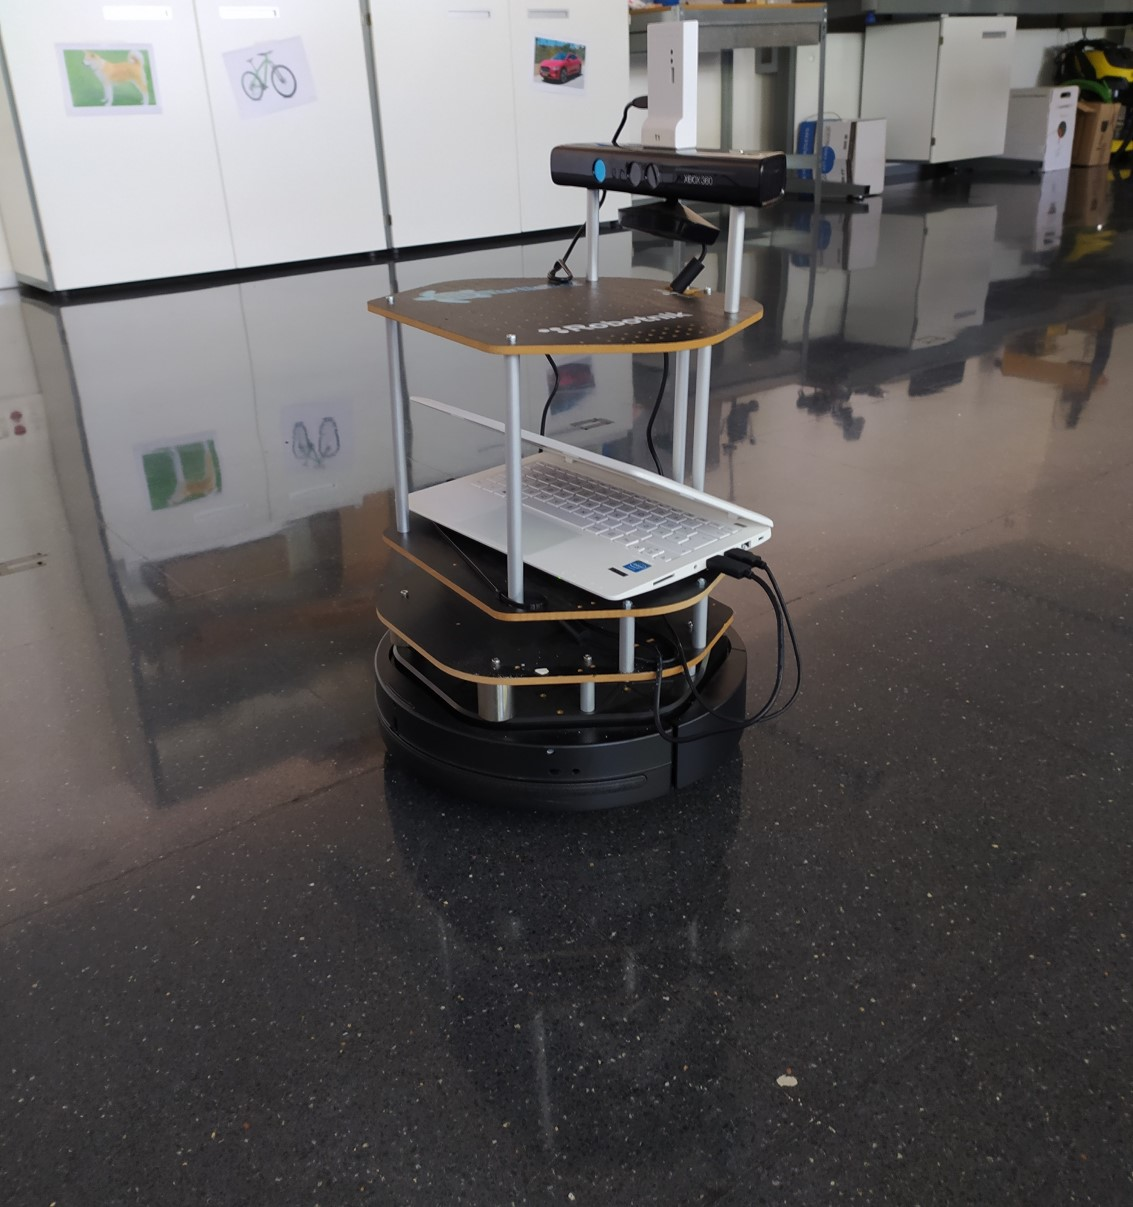
\includegraphics[width=0.55\textwidth]{pic/robot_lab.jpg}
    \caption{Turtlebot en una de las tomas de medidas.}
    \label{fig:robot}
\end{figure}

El TurtleBot funciona con ROS --\textit{Robot Operating System}, en inglés--, un entorno de trabajo enfocado a los sistemas robóticos encargado del soporte para todos los dispositivos hardware del robot como motores, encoders o cámaras. 
Cuenta con diversas librerías para distintos casos de uso, entre las que se encuentra la navegación en un entorno controlado como la que se da en el caso de este trabajo.

Su funcionamiento se basa en una arquitectura de grafos, donde se definen \textit{nodos}, tareas en las que se realiza el procesamiento de sensores, control, actuadores o cualquier otra función.
Los nodos se comunican entre ellos con mensajes llamados \textit{topic}, y es posible su desarrollo con los lenguajes C++ y Python.

Dentro de los paquetes disponibles, el usado en el desarrollo del trabajo es el encargado de la navegación del robot, que permite desplazar al robot a cualquier punto del entorno de trabajo y proporcionar de forma constante su posición en el mapa.

Es posible acoplar al robot un sistema de visión llamado Kinect que, mediante luz, permite obtener un mapa de profundidad del entorno que lo rodea.
Fue desarrollado en primera instancia para el uso en videojuegos pero su uso también se ha extendido a labores de investigación al permitir el posicionamiento de objetos y paredes, de tal manera que permite al robot evitar obstáculos dinámicos en el caso de que interpongan en su camino.

La funcionalidad de navegación aprovecha estos sensores realizando una fusión de sus resultados con los datos de movimiento de los motores que impulsan al robot, de tal forma que es posible corregir cualquier error en casos donde el empuje de las ruedas no se traslade directamente en un desplazamiento del robot, como puede ocurrir al rotar sobre sí mismo.

Para conseguir el posicionamiento en el mapa el paquete de navegación utiliza un \textit{planner} global sobre el que es posible determinar las rutas a seguir por el robot para llegar a un punto dado sorteando obstáculos y paredes.
Junto a él trabaja un \textit{planner} local, en el que gracias a los sensores incorporados se evalúan de forma continua los alrededores del robot.
Así, es posible conseguir de forma continua una evaluación de los posibles obstáculos que no se encuentran en el mapa del planner global, para lo que se construye un mapa de costes con el fin de abortar el movimiento en el caso de que sea imposible alcanzar el punto objetivo \cite{ROSDoc}.

Con la información actualizada del \textit{planner} local, el \textit{planner} global es capaz de modificar los trayectos para que el robot pueda continuar su desplazamiento por el mapa.
Es posible observar un esquema del funcionamiento de estos sistemas en la Figura~\ref{fig:move_base}.

\begin{figure}[H]
    \centering
    \def\svgwidth{0.8\linewidth}
    \input{./fig/navigation.pdf_tex}
	\caption{Esquema del funcionamiento del paquete de navegación de ROS.}
    \label{fig:move_base}
\end{figure}

Con esta herramienta la librería de navegación permite un mapeado autónomo tomando como referencia los datos de odometría que proporcionan los motores propulsores del robot para determinar las dimensiones del entorno.

En el caso de disponer de antemano de dichas dimensiones es posible proporcionar un mapa al sistema de navegación y evitar el paso de reconocimiento del entorno.
Esto no solo ahorra tiempo, sino que además minimiza las posibles discrepancias entre los datos de odometría y los desplazamientos reales del robot al realizar el mapeado de forma autónoma.

La opción de realizar un mapa previo fue la elegida en este caso, ya que el robot cuenta con rutinas para el reposicionamiento en el mapa en dicho caso.
Así, a partir de los límites establecidos y comprobados de forma manual, las posibles discrepancias en la odometría del robot se ven continuamente compensadas y corregidas.

A partir de estos datos corregidos es posible conocer en cualquier momento la posición del robot en el mapa, expuesta a través de ROS en uno de los topic disponibles.

Para facilitar el uso de ROS existe la posibilidad de usar el simulador Stage, capaz de crear un mundo virtual a partir de un mapa en dos dimensiones en el que colocar el Turtlebot y simular su funcionamiento de forma total sin tener acceso al robot de forma física.
Es posible observar su interfaz en la Figura~\ref{fig:stage_rviz}.

Además, ROS también permite el uso de una herramienta de visualización de la posición del robot en el mapa y de todos los sensores que incorpora llamada \textit{rviz}.
Aunque es compatible con Stage, sus funcionalidades brillan al usar el robot en entornos reales, donde es posible comprobar de forma continua que su posicionamiento es correcto y que sus sensores funcionan como es debido.


\begin{figure}[H] 
    \centering
    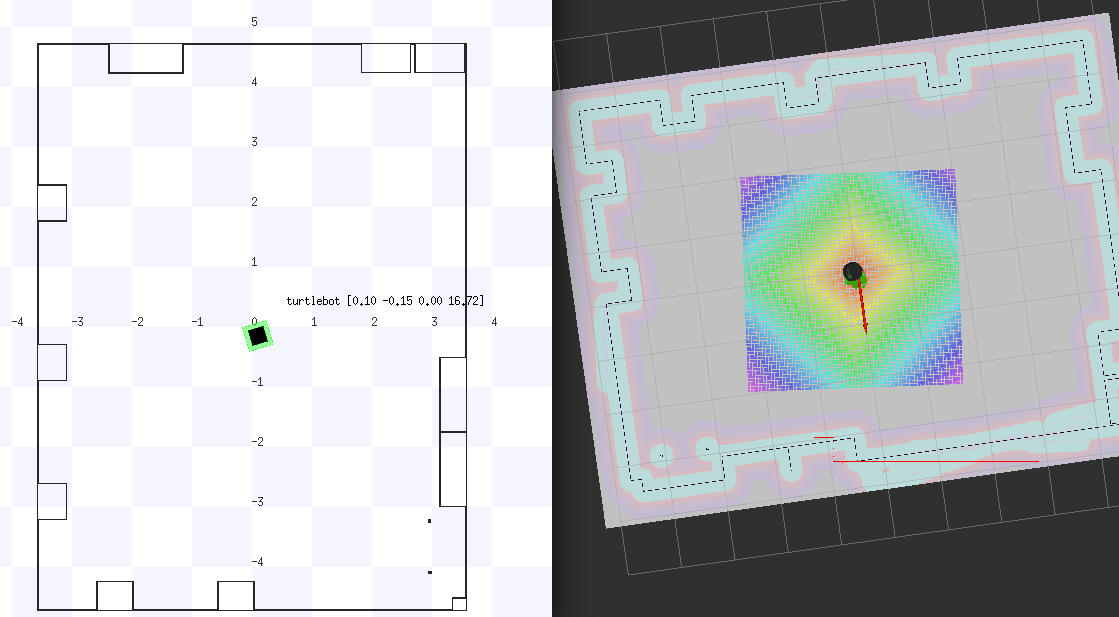
\includegraphics[width=0.75\textwidth]{pic/Stage-rviz.png}
    \caption{Captura del simulador Stage (a la izquierda) y la herramienta de visualización \textit{rviz} (a la derecha).}
    \label{fig:stage_rviz}
\end{figure}

\subsubsection{Trayectoria}

Dentro del laboratorio se eligió un área de $7 \times 5 \si{\meter}$ para el recorrido del robot, eligiendo los puntos en los que tomar las medidas separados 1 metro.

\begin{figure}[H]
    \begin{subfigure}[b]{.45\textwidth}
        \centering
        \def\svgwidth{0.6\linewidth}
	    \input{./fig/lab.pdf_tex} 
        \caption{Puntos a evaluar.}
        \label{fig:puntos}
    \end{subfigure}
    \begin{subfigure}[b]{.45\textwidth}
        \centering
        \def\svgwidth{0.6\linewidth}
	    \input{./fig/lab_vertical.pdf_tex} 
        \caption{Trayectoria del robot.}
        \label{fig:vertical}
    \end{subfigure}
    \caption{Puntos de medida por el robot en el laboratorio y la trayectoria tomada.}
    \label{fig:laboratorio}
\end{figure}

La Figura~\ref{fig:laboratorio} recoge la disposición de los puntos tomados y la ruta del robot para ello.
En total se compone de 35 puntos: en cada uno de ellos el robot se parará y tomará las 5 medidas correspodientes.

En todos los escenarios a comentar en la sección posterior la trayectoria fue la misma.
Si se coloca algún obstáculo en el camino del robot lo podrá evitar de forma totalmente autónoma, evitando tener que hacer cualquier modificación en la trayectoria establecida y programada.

\subsection{Escenarios}

Además del escenario del laboratorio sin ningún obstáculo, se utilizaron unas tablas de madera de dimensiones $1 \times 0.64 \times 0.02\si{\meter}$ forradas de forma parcial con papel de alumninio, de forma que pudieran presentar un cierto efecto de apantallamiento de la radiación en su dirección.

Estas tablas, colocadas en dos configuraciones, proporcionaron otros dos escenarios con obstáculos para comprobar de manera más profunda el comportamiento del simulador.

En todos los casos el emisor estuvo colocado en la misma posición: un metro por detrás del punto 2 tal y como se indica en la Figura~\ref{fig:laboratorio}, a $0.55\si{\centi\meter}$ de altura.

Es esta altura por la que solo se forra la mitad superior de las tablas: tal y como se mostraba en la sección~\ref{sec:antenas}, el patrón de emisión coloca la mayor parte de la potencia siendo emitida en el plano de la antena.
Sumando el mayor decaimiento al recorrer una distancia mayor, las trayectorias alternativas que involucren rebotes contra el suelo o el techo tendrán un efecto mucho menor, así que se conseguirá un apantallamiento suficiente con esta configuración.

\subsubsection{Escenario A}

El primer escenario fue la utilización del laboratorio sin ningún obstáculo, de forma que se espera que los rayos impacten únicamente contra las paredes, puertas y demás mobiliario que se queda fuera de la trayectoria del robot.

Por ello, en este caso predominará el efecto del decaimiento con la distancia, salvo en puntos cercanos a los límites del laboratorio.

\subsubsection{Escenario B}

Para un segundo escenario se colocó una tabla forrada tal y como se describía anteriormente.

Se colocó centrada horizontalmente, 1 metro por debajo del centro de la trayectoria como se muestra en la Figura~\ref{fig:escenarioB}.

\begin{figure}[H]
    \centering
    \begin{subfigure}[b]{0.45\textwidth}
        \centering
        % 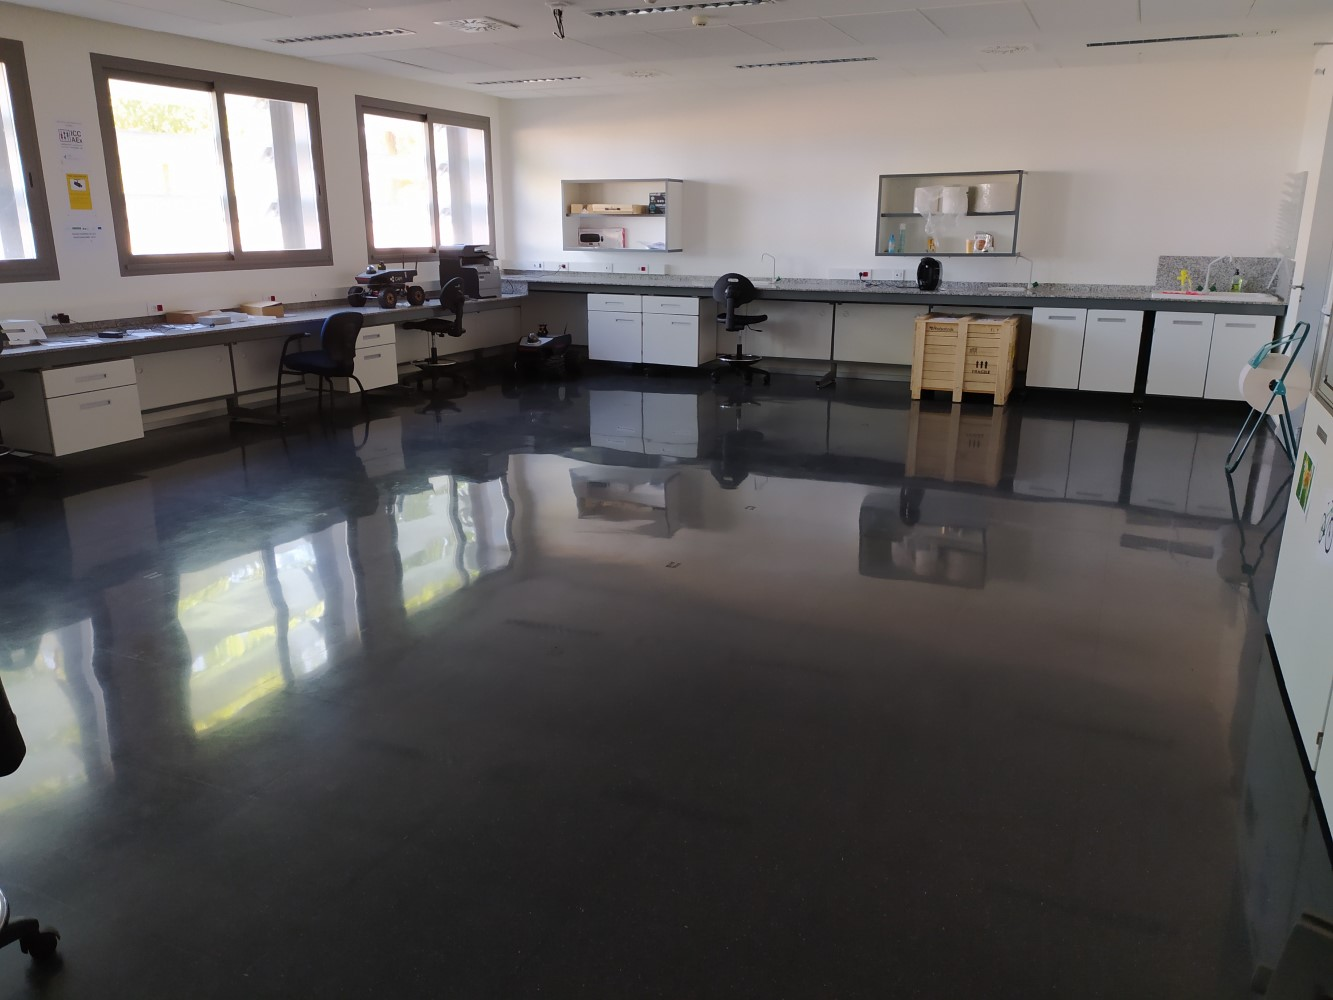
\includegraphics[width=6.8cm]{pic/lab1.jpg}
        \begin{tikzpicture}[scale=0.90]
    \draw (-2,-3) rectangle (2,3);

    \draw[thick] (-0.5, -1) -- (0.5, -1);

    \fill[black] (0,0) circle (0.05);

    \fill[red] (-1,-3.5) circle (0.075);

    \draw[<->] (0,-0.1) -- (0,-0.9);
    \node[anchor=west] at (0,-0.5) {1m};

    \draw[<->] (-1.75,-2.9) -- (-1.75,2.9);
    \node[anchor=west] at (-1.75,-2.5) {7m};

    \draw[<->] (-1.75, 2.7) -- (1.75, 2.7);
    \node[anchor=north] at (0, 2.7) {5m};
\end{tikzpicture}
        \caption{Esquema de la posición de la tabla. El punto rojo indica la posición del emisor.}
        % \label{fig:antena_router}
    \end{subfigure}
    ~~
    \begin{subfigure}[b]{0.45\textwidth}
        \centering
        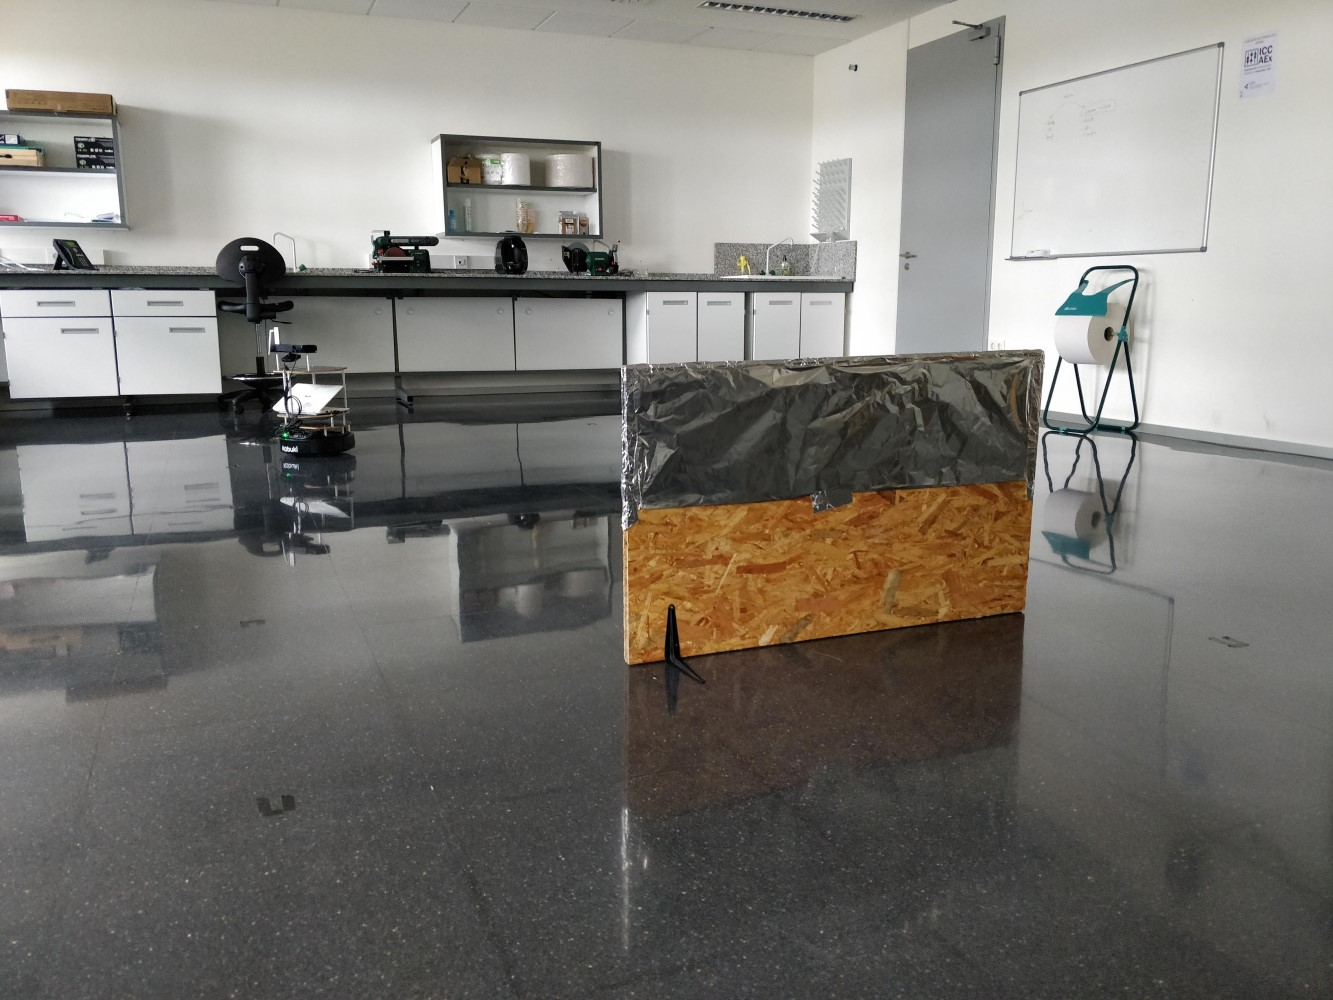
\includegraphics[width=6.8cm]{pic/escB.jpg}
        \caption{Imagen del laboratorio en el escenario B.}
        % \label{fig:antena_receptor}
    \end{subfigure}
    \caption{Diposición en el escenario B.}
    \label{fig:escenarioB}
\end{figure}

En este caso se busca que la tabla presente un efecto atenuante en toda la zona detrás de la tabla, creando una zona diagonal donde se deberían obtener valores de potencia menores que en el escenario A.

\subsubsection{Escenario C}

El tercer y último escenario tiene en cuenta dos tablas, esta vez colocadas con una orientación distinta.

Se colocan en este caso dos tablas a $1.5$ metros del centro de distancia horizontal, a ambos lados.
En cuanto a la distancia vertical, una de ellas se coloca a $1.5$ metros por encima y la otra la misma distancia por debajo. --donde esta orientación hace referencia a la distribución indicada en la Figura~\ref{fig:escenarioC}--.

\begin{figure}[H]
    \centering
    \begin{subfigure}[b]{0.45\textwidth}
        \centering
        % 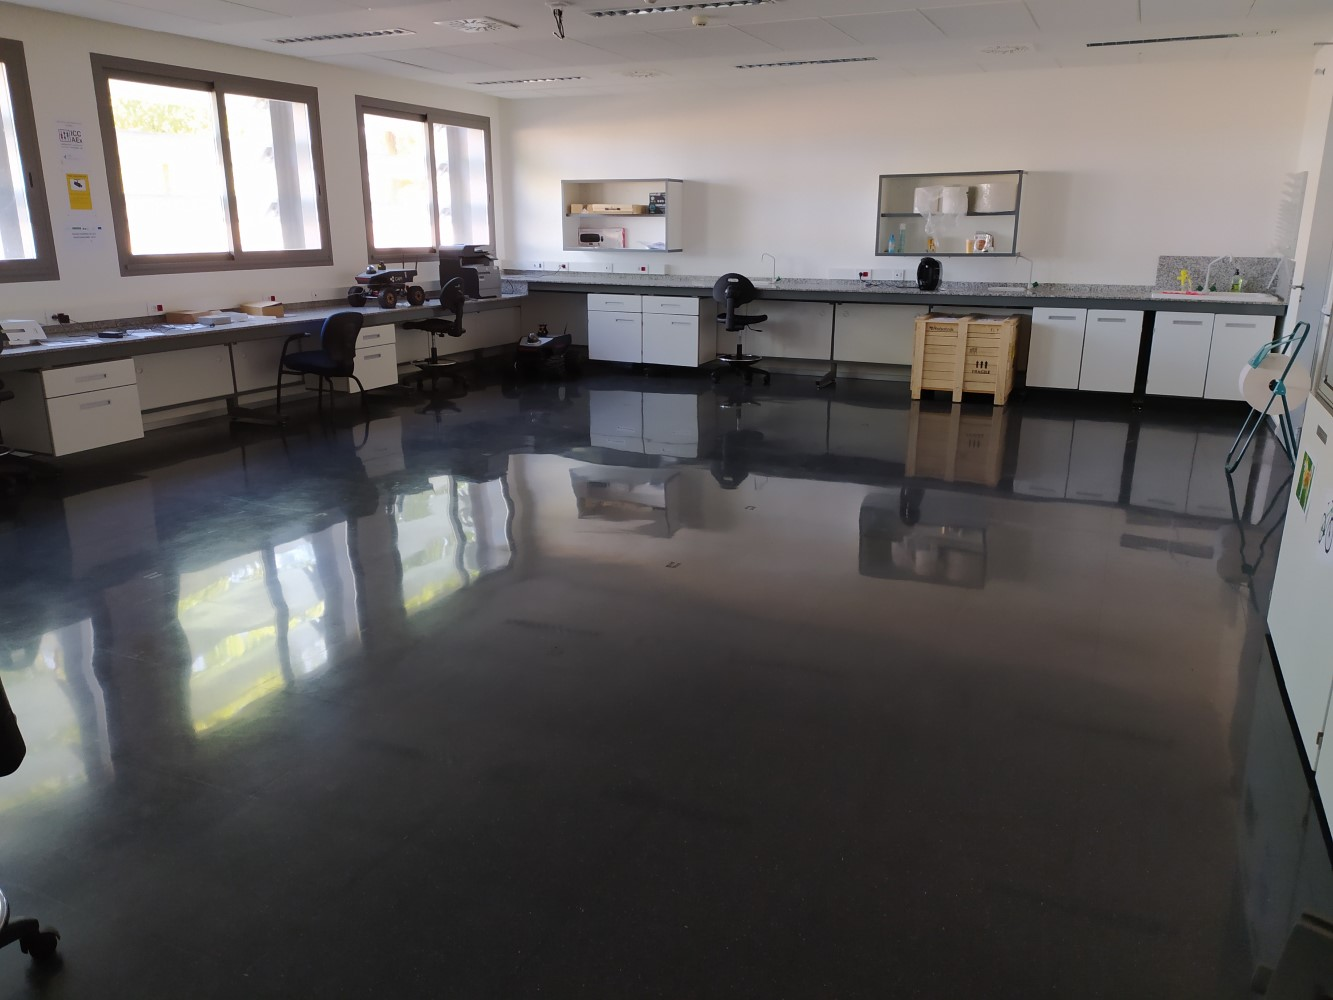
\includegraphics[width=6.8cm]{pic/lab1.jpg}
        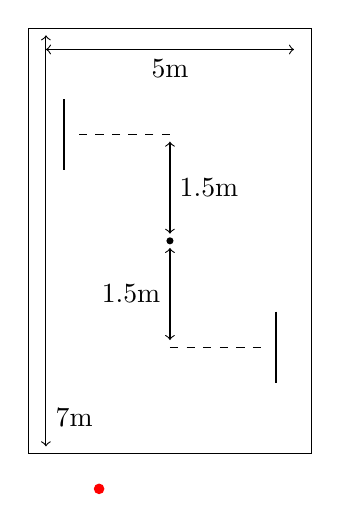
\begin{tikzpicture}[scale=0.90]
    \draw (-2,-3) rectangle (2,3);

    \draw[thick] (-1.5, 1) -- (-1.5, 2);
    \draw[thick] (1.5, -1) -- (1.5, -2);

    \fill[black] (0,0) circle (0.05);

    \fill[red] (-1,-3.5) circle (0.075);

    \draw[<->] (0,-0.1) -- (0,-1.4);
    \draw[dashed] (0, -1.5) -- (1.4, -1.5);
    \node[anchor=east] at (0,-0.75) {1.5m};

    \draw[<->] (0, 0.1) -- (0, 1.4);
    \draw[dashed] (0, 1.5) -- (-1.4, 1.5);
    \node[anchor=west] at (0, 0.75) {1.5m};

    \draw[<->] (-1.75,-2.9) -- (-1.75,2.9);
    \node[anchor=west] at (-1.75,-2.5) {7m};

    \draw[<->] (-1.75, 2.7) -- (1.75, 2.7);
    \node[anchor=north] at (0, 2.7) {5m};
\end{tikzpicture}
        \caption{Esquema de la posición de las tablas. El punto rojo indica la posición del emisor.}
        % \label{fig:antena_router}
    \end{subfigure}
    ~~
    \begin{subfigure}[b]{0.45\textwidth}
        \centering
        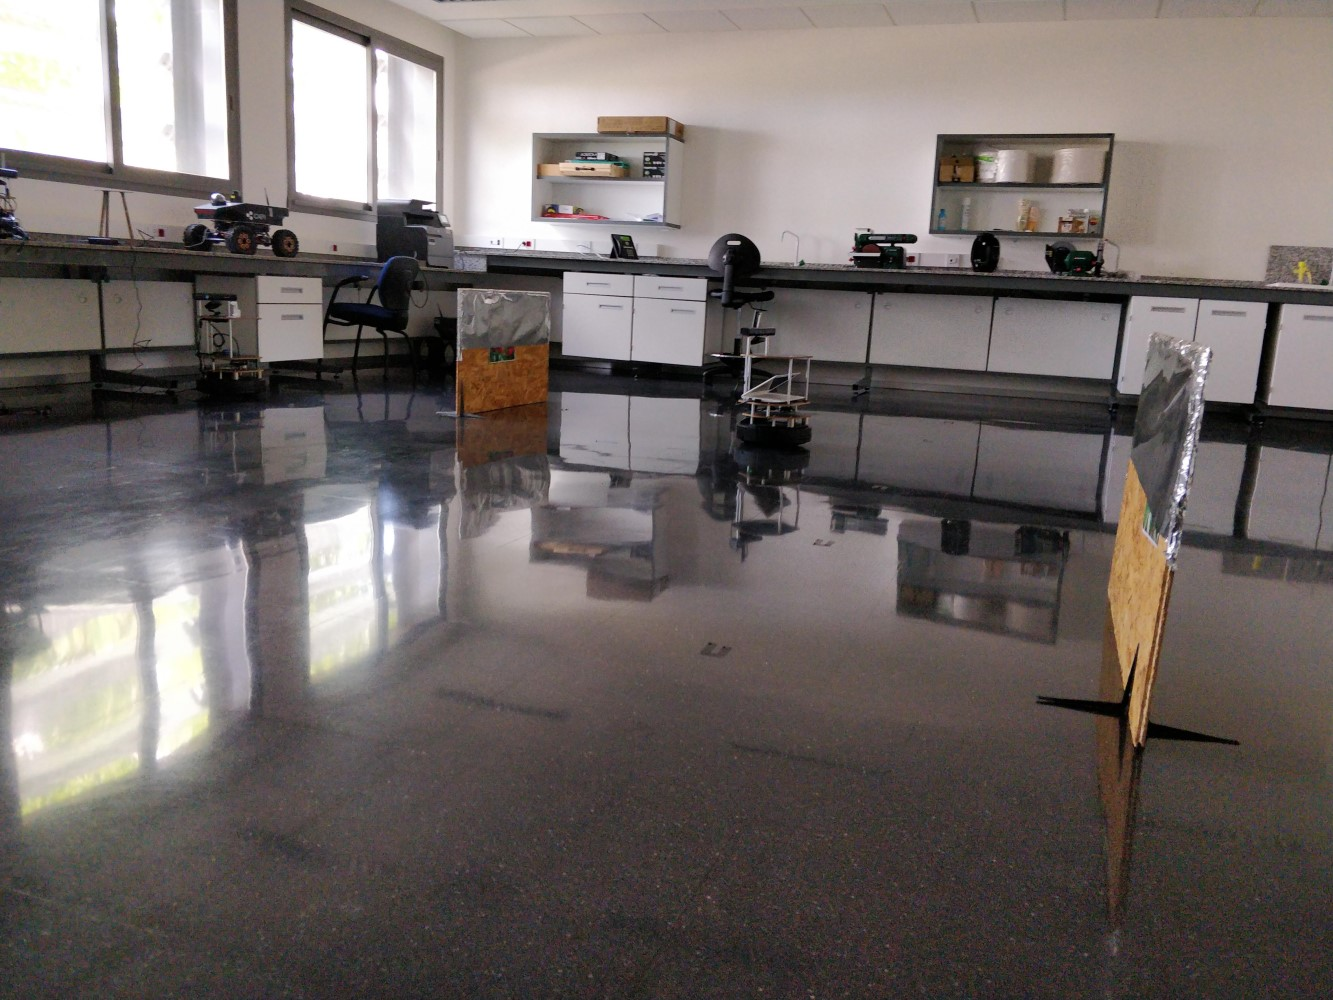
\includegraphics[width=6.8cm]{pic/escC.jpg}
        \caption{Imagen del laboratorio en el escenario C.}
        % \label{fig:antena_receptor}
    \end{subfigure}
    \caption{Diposición en el escenario C.}
    \label{fig:escenarioC}
\end{figure}

A diferencia del caso anterior, en este escenario no se busca tanto el apantallamiento --aunque puede haberlo-- sino el efecto de los rebotes.

Así, se espera que en la parte central pueda haber una potencia algo mayor que en el escenario A, aunque no debería haber un aumento significativo debido a la mayor distancia recorrida por los ángulos y el rebote que sufren.

